\chapter{Metodologia} \label{Cap:Metodologia}

Este trabalho adota uma abordagem quantitativa de natureza aplicada, fundamentada na construção e avaliação experimental de modelos preditivos de customer churn. O estudo compreende cinco etapas sequenciais, detalhadas ao longo deste capítulo e do Capítulo \ref{Cap:AvaliacaoExperimental}: (i) carregamento e integração dos dados; (ii) engenharia de features com janela temporal anti-leakage; (iii) definição do target e estratégia de balanceamento de classes; (iv) treinamento e avaliação comparativa de dez algoritmos de Machine Learning; e (v) análise de importância de features, valores SHAP e segmentação de risco dos clientes. A Figura \ref{fig:pipeline} sintetiza o encadeamento dessas etapas.

\begin{figure}[H]
\caption{Pipeline metodológico do estudo}
\label{fig:pipeline}
\begin{center}
	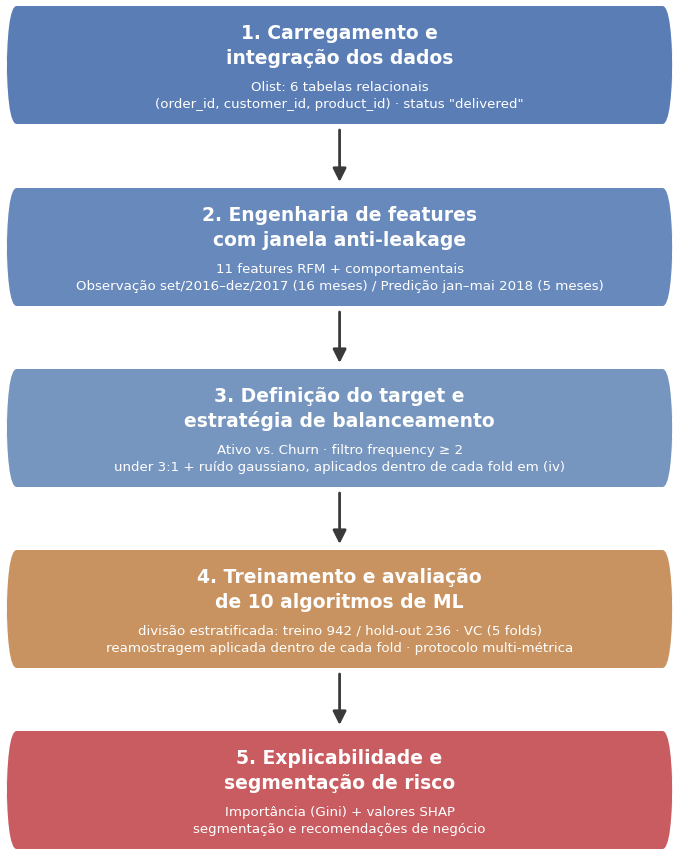
\includegraphics[width=0.6\textwidth]{USPSC-img/figuras/fig01-pipeline.png}
\end{center}
\begin{flushleft}
	\ABNTEXfontereduzida
	\SingleSpacing
	Fonte: elaborado pelo autor.

	\textit{Nota: a estratégia de balanceamento é definida na etapa (3) e aplicada na etapa (4), dentro de cada partição da validação cruzada, conforme o protocolo descrito na Seção \ref{sec:protocolo}.}
\end{flushleft}
\end{figure}

\FloatBarrier
\section{Base de Dados e Integração} \label{sec:base-dados}

A base de dados utilizada é o Olist Brazilian E-Commerce Public Dataset \cite{olist2018}, composto por seis tabelas relacionais: pedidos, clientes, itens de pedido, pagamentos, avaliações e produtos. A integração das tabelas foi realizada por meio de chaves primárias e estrangeiras compartilhadas (order\_id, customer\_id e product\_id), resultando em um dataset unificado cujo período de cobertura, conforme a documentação do conjunto de dados \cite{olist2018}, estende-se de setembro de 2016 a outubro de 2018. Foram considerados exclusivamente pedidos com status ``delivered'', garantindo que apenas transações efetivamente concluídas compusessem a base de análise.

\FloatBarrier
\section{Estratégia Temporal Anti-Leakage} \label{sec:janela-temporal}

A fim de evitar o vazamento de informação futura para o conjunto de treino, problema conhecido como data leakage, adotou-se uma estratégia de janela temporal dupla. A janela de observação, na qual as features comportamentais de cada cliente são computadas, encerra-se em 31 de dezembro de 2017 e abrange todo o histórico transacional disponível até essa data (setembro de 2016 a dezembro de 2017, aproximadamente dezesseis meses), assegurando suficiência estatística e contemplando um ciclo sazonal completo. A janela de predição, de 1.\textsuperscript{o} de janeiro a 31 de maio de 2018, define o período no qual se verifica se o cliente realizou nova compra, determinando, assim, sua classificação como Ativo (retornou) ou Churn (não retornou). Essa separação temporal garante que nenhuma informação posterior ao momento de predição influencie os modelos.

A escolha do horizonte de predição foi deliberada: cinco meses equilibram sensibilidade à recompra e representatividade do horizonte preditivo, janela compatível com um contexto de e-commerce marcado pela predominância de clientes de compra única, característica documentada para o mesmo dataset por \citeonline{matuszelanski2022}. A Figura \ref{fig:janela-temporal} representa graficamente essa separação temporal.

\begin{figure}[htbp]
\caption{Estratégia de janela temporal dupla (anti-leakage)}
\label{fig:janela-temporal}
\begin{center}
	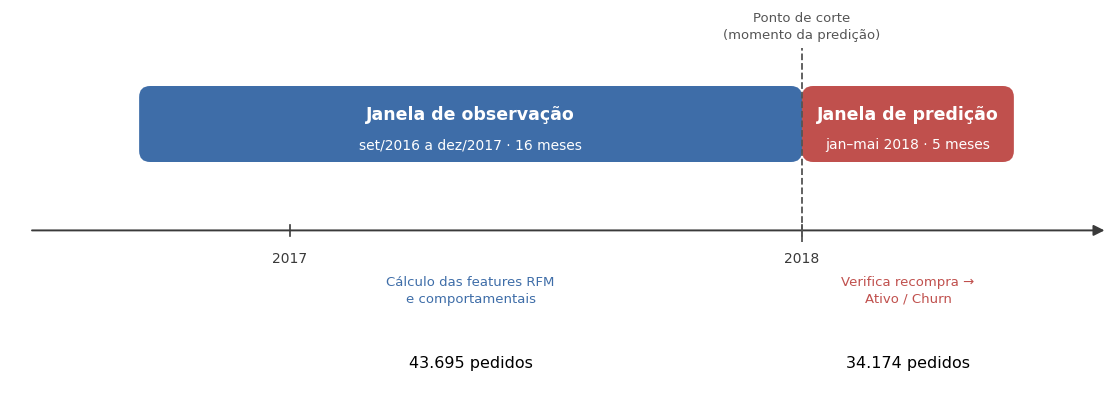
\includegraphics[width=1\textwidth]{USPSC-img/figuras/fig02-janela-temporal.png}
\end{center}
\begin{flushleft}
	\ABNTEXfontereduzida
	\SingleSpacing
	Fonte: elaborado pelo autor.
\end{flushleft}
\end{figure}

\FloatBarrier
\section{Engenharia de Features RFM} \label{sec:engenharia-features}

Com base na janela de observação, foram calculadas onze features por cliente, seguindo a metodologia RFM e incluindo variáveis complementares de comportamento transacional. A Tabela \ref{tab:features-rfm} sumariza as features construídas.

\begin{table}[htbp]
\ABNTEXfontereduzida
\SingleSpacing
\caption{Features RFM construídas na janela de observação (até dez/2017)}
\label{tab:features-rfm}
\centering
\begin{tabular}{l l l}
\hline
\textbf{Feature} & \textbf{Tipo} & \textbf{Descrição / Fórmula} \\
\hline
\textit{recency\_days}        & Numérica   & 01/01/2018 $-$ data do último pedido (em dias) \\
\textit{frequency}            & Numérica   & COUNT(DISTINCT order\_id) por customer\_unique\_id \\
\textit{monetary}             & Numérica   & SUM(valor do pedido) por customer\_unique\_id \\
\textit{avg\_ticket}          & Numérica   & monetary / frequency \\
\textit{avg\_delivery\_days}  & Numérica   & MEAN(data\_entrega $-$ data\_compra) \\
\textit{avg\_review\_score}   & Numérica   & MEAN(review\_score) \\
\textit{avg\_installments}    & Numérica   & MEAN(payment\_installments) \\
\textit{avg\_freight}         & Numérica   & MEAN(freight\_value) \\
\textit{n\_categories}        & Numérica   & COUNT(DISTINCT product\_category\_name) \\
\textit{top\_category}        & Categórica & MODE(product\_category\_name) $\rightarrow$ Label Encoding \\
\textit{customer\_state}      & Categórica & UF do cliente $\rightarrow$ Label Encoding \\
\hline
\end{tabular}
\begin{flushleft}
	\ABNTEXfontereduzida
	\SingleSpacing
	Fonte: elaborado pelo autor.

	\textit{Nota: registros sem categoria de produto identificada, correspondentes a 1,8\% do conjunto integrado, recebem o rótulo ``desconhecido'' na etapa de construção das features (Seção \ref{sec:protocolo}). Esse rótulo é computado como categoria distinta por COUNT(DISTINCT product\_category\_name), de modo que clientes com pedidos nessa condição podem ter a contagem de n\_categories acrescida em uma unidade.}
\end{flushleft}
\end{table}

As nove features numéricas cobrem as três dimensões do RFM e derivadas do comportamento transacional, conforme detalhado na Tabela \ref{tab:features-rfm}. As features categóricas compreendem top\_category e customer\_state, ambas submetidas a Label Encoding antes do treinamento. A opção pela codificação ordinal, em detrimento da codificação binária por one-hot, decorre da cardinalidade dessas variáveis frente ao tamanho da base: o catálogo de produtos do dataset contém 73 categorias distintas, às quais se soma o rótulo ``desconhecido'', de modo que a expansão binária elevaria a dimensionalidade a patamar incompatível com 1.178 observações. Cabe registrar a limitação inerente à escolha: modelos baseados em árvores tratam o inteiro atribuído a cada categoria como grandeza ordenada, produzindo partições sobre uma ordem que não possui significado substantivo. Esse efeito soma-se ao viés da importância por impureza de Gini em variáveis categóricas de cardinalidade elevada, discutido na Seção \ref{sec:interpretabilidade}, e recomenda cautela na interpretação da posição de top\_category nos rankings de importância. Codificações alternativas são registradas entre os trabalhos futuros. Clientes com frequency igual a 1 foram excluídos do escopo de modelagem, pois compradores únicos não possuem histórico suficiente para caracterizar comportamento de recompra e sua inclusão trivializaria o target Churn sem adicionar poder preditivo real.

Essa decisão de filtragem foi submetida à validação empírica no notebook que acompanha esta monografia: um modelo Random Forest de referência foi treinado em duas configurações, com o filtro adotado (frequency $\geq$ 2; 1.178 clientes) e incluindo os compradores únicos (frequency $\geq$ 1; mais de 42 mil clientes, com 98,9\% de Churn). A inclusão dos compradores únicos reduziu o ROC-AUC em aproximadamente 0,29 ponto (de 0,8106 para 0,5231), aproximando o modelo de um classificador aleatório, e degradou o MCC em cerca de 79\% (de 0,1931 para 0,0400). O resultado confirma empiricamente que os compradores únicos não agregam sinal preditivo de recompra, apenas diluem o problema, corroborando a recomendação de \citeonline{matuszelanski2022} para o dataset Olist.

A feature n\_categories foi incluída por hipótese de negócio (clientes que diversificam categorias demonstram maior engajamento com a plataforma), em linha com as recomendações de \citeonline{manzoor2024} sobre variáveis comportamentais complementares ao RFM. A variável revelou-se, posteriormente, um dos três principais drivers preditivos do modelo, em empate técnico de importância com a recência. Tal equivalência entre diversidade de categorias e recência não é reportada nos estudos anteriores aplicados ao Olist, incluindo \citeonline{matuszelanski2022}. Sua relevância sugere que a diversificação de categorias merece investigação como possível alavanca de retenção proativa, hipótese a ser confirmada em bases de maior volume.

\FloatBarrier
\section{Target e Balanceamento de Classes} \label{sec:target-balanceamento}

O target binário foi definido como: Churn = 1 para clientes que não realizaram nenhuma compra na janela de predição; e Ativo = 0 para aqueles que efetuaram ao menos uma transação no período. A base resultante apresentou desbalanceamento acentuado, com 95,8\% dos clientes classificados como Churn e 4,2\% como Ativos. Cabe destacar que essa proporção se verifica em uma coorte composta exclusivamente por clientes recorrentes, o que evidencia que, mesmo entre consumidores com histórico de recompra, os intervalos entre transações tendem a exceder o horizonte de predição adotado, característica consistente com a baixa taxa de retorno documentada para o dataset Olist \cite{matuszelanski2022}.

Para mitigar o efeito do desbalanceamento extremo, que tende a produzir modelos enviesados para a classe majoritária e com baixa capacidade preditiva real \cite{he2009}, adotou-se uma estratégia combinada de under e oversampling aplicada exclusivamente ao conjunto de treino. O undersampling reduziu a classe majoritária (Churn) a no máximo três vezes o tamanho da classe minoritária (Ativo). O oversampling sintético por ruído gaussiano de média zero e desvio-padrão 0,05, aplicado sobre as features já padronizadas (média 0, desvio padrão 1), expandiu a classe Ativo até igualar o tamanho da maioria, produzindo um conjunto de treino perfeitamente balanceado. Não se trata de interpolação entre vizinhos, como no SMOTE: cada instância sintética é uma cópia de uma observação real da classe minoritária somada a perturbação de baixa magnitude, procedimento que preserva a vizinhança original em vez de criar pontos em regiões não observadas do espaço de features. O procedimento corresponde à replicação ruidosa (\textit{noisy replication}) formulada por \citeonline{lee2000} para classificação binária com classes assimétricas, e encontra respaldo teórico no resultado de \citeonline{bishop1995}, segundo o qual o treinamento com ruído aditivo de baixa variância equivale a uma forma de regularização de Tikhonov, o que explica por que a perturbação atua como regularizador em vez de introduzir ruído estrutural. O conjunto de teste foi mantido com a distribuição original, preservando a validade da avaliação.

Essa escolha se apoiou em uma análise comparativa sistemática das alternativas de tratamento do desbalanceamento, sintetizada no Quadro \ref{qua:estrategias-balanceamento}, que pondera vantagens e riscos de cada estratégia à luz do tamanho reduzido da classe minoritária (aproximadamente 50 clientes ativos). Optou-se pela combinação de undersampling moderado (razão 3:1) com oversampling gaussiano por preservar a vizinhança real dos dados sem descartar informação da classe majoritária nem gerar instâncias em regiões não representativas, como poderia ocorrer com o SMOTE \cite{chawla2002} em um conjunto tão pequeno e esparso. Trata-se, portanto, de alternativa deliberadamente mais conservadora, cuja adequação foi verificada empiricamente por meio da análise de representatividade conduzida na Seção \ref{sec:representatividade}.

\begin{quadro}[htbp]
\ABNTEXfontereduzida
\SingleSpacing
\caption{Análise comparativa de estratégias de balanceamento de classes}
\label{qua:estrategias-balanceamento}
\centering
\begin{tabular}{|>{\raggedright\arraybackslash}p{3.0cm}|>{\raggedright\arraybackslash}p{5.3cm}|>{\raggedright\arraybackslash}p{5.6cm}|}
\hline
\textbf{Estratégia} & \textbf{Vantagens} & \textbf{Desvantagens / Riscos} \\
\hline
Sem balanceamento & Preserva a distribuição real; sem artefatos sintéticos. & Modelos enviesados para a classe majoritária, com regra de decisão que só alcança recall não trivial na classe Ativo mediante limiar muito acima do padrão (0,75 na Tabela \ref{tab:comparacao-balanceamento}). \\
\hline
Undersampling puro & Simples; reduz custo computacional; sem dados sintéticos. & Descarta a quase totalidade da classe Churn; base de treino diminuta (cerca de 80 amostras) com 40 Ativos. \\
\hline
SMOTE (oversampling sintético) & Amplia a classe minoritária por interpolação entre vizinhos reais; consagrado na literatura. & Em datasets pequenos e esparsos, gera instâncias em regiões não representativas; risco de ruído estrutural. \\
\hline
\textbf{Under + oversampling gaussiano (adotada)} & Equilibra as classes; retém três vezes mais amostras Churn que o undersampling puro; perturbação de baixa magnitude preserva a vizinhança real. & Ainda descarta cerca de 87\% da classe Churn presente no conjunto de treino; dois terços da classe Ativo no treino são sintéticos; exige validação de representatividade (Seção \ref{sec:representatividade}). \\
\hline
\end{tabular}
\begin{flushleft}
	\ABNTEXfontereduzida
	\SingleSpacing
	Fonte: elaborado pelo autor.
\end{flushleft}
\end{quadro}

\begin{table}[htbp]
\ABNTEXfontereduzida
\SingleSpacing
\caption{Comparação empírica de estratégias de balanceamento (split de referência)}
\label{tab:comparacao-balanceamento}
\centering
\scriptsize
\setlength{\tabcolsep}{3pt}
\begin{tabular}{@{}>{\raggedright\arraybackslash}p{3.0cm}rrrrrrrrr@{}}
\hline
\textbf{Estratégia} & \shortstack[r]{\textbf{N}\\\textbf{treino}} & \shortstack[r]{\textbf{ROC-}\\\textbf{AUC}} & \shortstack[r]{\textbf{CV-}\\\textbf{AUC}} & \textbf{MCC} & \textbf{Kappa} & \shortstack[r]{\textbf{F1-}\\\textbf{Macro}} & \shortstack[r]{\textbf{Rec.}\\\textbf{Ativo}} & \shortstack[r]{\textbf{Rec.}\\\textbf{Churn}} & \textbf{Limiar} \\
\hline
Sem balanceamento & 942 & 0,8018 & 0,6017 & 0,2983 & 0,2680 & 0,6319 & 0,20 & 0,9912 & 0,75 \\
Undersampling puro (1:1) & 80 & 0,7451 & 0,6080 & 0,1943 & 0,1884 & 0,5930 & 0,30 & 0,9425 & 0,27 \\
SMOTE & 1.804 & 0,7327 & 0,5928 & 0,1253 & 0,1233 & 0,5610 & 0,20 & 0,9469 & 0,44 \\
\textbf{Under 3:1 + gaussiano (adotada)} & \textbf{240} & \textbf{0,8106} & \textbf{0,6814} & \textbf{0,1931} & \textbf{0,1918} & \textbf{0,5957} & \textbf{0,20} & \textbf{0,9735} & \textbf{0,38} \\
\hline
\end{tabular}
\begin{flushleft}
	\ABNTEXfontereduzida
	\SingleSpacing
	Fonte: elaborado pelo autor.

	\textit{Nota: modelo de referência Random Forest (n\_estimators = 300, max\_depth = 10), mantido fixo nas quatro estratégias; o que se compara aqui são estratégias de reamostragem, não algoritmos. A reamostragem é aplicada dentro de cada partição da validação cruzada, e o limiar de classificação é derivado das probabilidades out-of-fold do conjunto de treino, conforme o protocolo descrito na Seção \ref{sec:protocolo}. Como o limiar é derivado independentemente em cada estratégia, as métricas dependentes de limiar (MCC, Kappa, F1-Macro e os recalls) são calculadas em pontos de corte distintos e não constituem comparação direta entre estratégias; a comparação estritamente pareada é a das colunas ROC-AUC e CV-AUC.}
\end{flushleft}
\end{table}

\begin{table}[htbp]
\ABNTEXfontereduzida
\SingleSpacing
\caption{Robustez das estratégias de balanceamento em trinta divisões estratificadas}
\label{tab:robustez-balanceamento}
\centering
\scriptsize
\setlength{\tabcolsep}{4pt}
\begin{tabular}{@{}>{\raggedright\arraybackslash}p{4.0cm}rrrr@{}}
\hline
\textbf{Estratégia} & \shortstack[r]{\textbf{ROC-AUC}\\\textbf{média}} & \shortstack[r]{\textbf{MCC}\\\textbf{médio}} & \shortstack[r]{\textbf{Kappa}\\\textbf{médio}} & \shortstack[r]{\textbf{Amplitude da}\\\textbf{ROC-AUC}} \\
\hline
Sem balanceamento & 0,6543 $\pm$ 0,0778 & 0,1168 $\pm$ 0,1167 & 0,1031 $\pm$ 0,1004 & 0,462 - 0,800 \\
Undersampling puro (1:1) & 0,6510 $\pm$ 0,0769 & 0,0439 $\pm$ 0,0765 & 0,0392 $\pm$ 0,0689 & 0,501 - 0,802 \\
SMOTE & 0,6615 $\pm$ 0,0660 & 0,1060 $\pm$ 0,0761 & 0,0895 $\pm$ 0,0696 & 0,539 - 0,810 \\
\textbf{Under 3:1 + gaussiano (adotada)} & \textbf{0,6686 $\pm$ 0,0831} & \textbf{0,1140 $\pm$ 0,0804} & \textbf{0,1053 $\pm$ 0,0726} & \textbf{0,500 - 0,822} \\
\hline
\end{tabular}
\begin{flushleft}
	\ABNTEXfontereduzida
	\SingleSpacing
	Fonte: elaborado pelo autor.

	\textit{Nota: aplica-se aqui a mesma observação da Tabela \ref{tab:comparacao-balanceamento} quanto ao modelo de referência e ao protocolo de avaliação.}
\end{flushleft}
\end{table}

A comparação empírica das quatro estratégias, conduzida no notebook que acompanha esta monografia e sintetizada nas Tabelas \ref{tab:comparacao-balanceamento} e \ref{tab:robustez-balanceamento}, corrobora a escolha adotada. No split de referência, a combinação de undersampling moderado com oversampling gaussiano obteve a maior ROC-AUC (0,811), à frente da ausência de balanceamento (0,802), do undersampling puro (0,745) e do SMOTE (0,733). Para verificar se esse resultado não decorria de uma partição favorável, o experimento foi repetido em trinta divisões estratificadas independentes, nas quais a estratégia adotada manteve a maior ROC-AUC média (0,669), seguida pelo SMOTE (0,662), pela ausência de balanceamento (0,654) e pelo undersampling puro (0,651).

O desempenho inferior do undersampling puro é consistente com a redução drástica do conjunto de treino que a estratégia impõe: com apenas 40 clientes Ativos no treino, o balanceamento 1:1 produz 80 amostras, base insuficiente para algoritmos ensemble. O SMOTE \cite{chawla2002}, por sua vez, interpola entre vizinhos reais, procedimento que em conjuntos pequenos e esparsos tende a gerar instâncias em regiões pouco representativas do espaço de features. A ausência de balanceamento, embora competitiva em ROC-AUC, preserva o viés estrutural para a classe majoritária que a literatura documenta em cenários de desbalanceamento extremo \cite{he2009}.

Cabe registrar duas ressalvas. A primeira é que, segundo o Coeficiente de Correlação de Matthews, uma das três métricas recomendadas por De la Cruz Huayanay, Bazán e Russo (\citeyear{delacruz2025}), a ausência de balanceamento supera a estratégia adotada no split de referência (0,2983 contra 0,1931, Tabela \ref{tab:comparacao-balanceamento}). O mesmo se verifica no Kappa de Cohen (0,2680 contra 0,1918) e no F1-Macro (0,6319 contra 0,5957), ambos igualmente favoráveis à ausência de balanceamento nesse split. Cabe observar, contudo, que essa vantagem não se traduz em ganho na classe minoritária: ambas as estratégias identificam corretamente a mesma proporção de clientes Ativos (Recall-Ativo de 0,20), e a diferença de MCC decorre exclusivamente do desempenho na classe majoritária (Recall-Churn de 0,9912 contra 0,9735). Na média das trinta divisões independentes, a diferença praticamente desaparece (MCC de 0,1140 para a estratégia adotada contra 0,1168 para a ausência de balanceamento, com desvios-padrão de 0,0804 e 0,1167), e a estratégia adotada apresenta o maior Kappa médio do conjunto (0,1053). A segunda ressalva é que as diferenças entre as estratégias situam-se dentro de um desvio-padrão, de modo que os resultados indicam tendência, e não superioridade estatisticamente estabelecida. A amplitude da ROC-AUC entre divisões, de 0,500 a 0,822 para a estratégia adotada, decorre do tamanho reduzido da classe Ativo no conjunto de teste (aproximadamente dez instâncias), limitação inerente ao problema e discutida ao longo deste trabalho. Reconhece-se, por fim, que o oversampling por ruído amplia a classe minoritária a partir de uma base amostral reduzida, o que motiva a análise de representatividade conduzida na Seção \ref{sec:representatividade}.

\FloatBarrier
\section{Protocolo de Treinamento e Avaliação} \label{sec:protocolo}

Os dados foram divididos em treino (80\%) e teste (20\%) por meio de StratifiedShuffleSplit, garantindo a proporção original de classes em ambos os conjuntos. A imputação de valores ausentes no conjunto de modelagem foi realizada pela mediana das features numéricas, e a padronização foi aplicada via StandardScaler, com parâmetros ajustados exclusivamente no conjunto de treino para evitar contaminação do teste \cite{kaufman2012}.

Precede essa etapa o tratamento de ausências na construção das features, integralmente contido na janela de observação e, portanto, anterior à definição do target e sem acesso a informação da janela de predição. Nesse tratamento, as variáveis de valor de pagamento e de avaliação foram imputadas pela mediana da respectiva coluna; as variáveis de frete e de número de parcelas receberam os valores neutros zero e um; e a categoria do produto, ausente em 1,8\% dos registros do conjunto integrado, recebeu o rótulo ``desconhecido'', conforme registrado na nota da Tabela \ref{tab:features-rfm}.

Foram treinados e avaliados dez algoritmos de Machine Learning: Regressão Logística, Árvore de Decisão, Random Forest, Extra Trees, Gradient Boosting, HistGradient Boosting, AdaBoost, K-Nearest Neighbors (KNN), Gaussian Naive Bayes e Support Vector Machine (SVM). Cada modelo foi submetido a validação cruzada estratificada com cinco folds (StratifiedKFold) no conjunto de treino e avaliado no hold-out de teste. A imputação, a padronização e a reamostragem são ajustadas dentro de cada partição, exclusivamente sobre a porção de ajuste, procedimento necessário para que instâncias sintéticas derivadas de uma mesma observação original não se distribuam entre folds distintos \cite{hastie2009,kaufman2012}. Registra-se que parte dos estimadores mantém o parâmetro class\_weight = ``balanced'' por padrão defensivo; sob o conjunto de treino perfeitamente balanceado (120/120), o parâmetro atribui pesos iguais às classes e é, portanto, neutro.

O protocolo de avaliação adota um conjunto abrangente de métricas sensíveis ao desbalanceamento, incorporando as três recomendadas por De la Cruz Huayanay, Bazán e Russo (\citeyear{delacruz2025}), a saber, MCC (Coeficiente de Correlação de Matthews), G-Mean e Kappa de Cohen, além de ROC-AUC, Average Precision, F1-Macro, Precisão e Recall por classe. Adota-se a classe Churn como positiva em todas as métricas por classe e na leitura da matriz de confusão, de modo que falso positivo designa cliente Ativo classificado como Churn, e falso negativo, cliente Churn classificado como Ativo.

O limiar de classificação constitui parâmetro livre da regra de decisão e, como tal, deve ser estimado sobre dados que não participem do relato de desempenho; estimá-lo no conjunto de teste equivale a utilizá-lo duas vezes, uma para ajustar o parâmetro e outra para reportar o resultado, o que caracteriza viés de seleção na avaliação \cite{cawley2010,hastie2009}. Dado que o valor padrão de 0,50 raramente é ótimo \cite{fawcett2006} e que o tamanho da classe minoritária inviabiliza a extração de uma terceira partição de validação, adotou-se o seguinte procedimento: as probabilidades preditas foram obtidas por validação cruzada estratificada de cinco folds sobre o conjunto de treino, com a reamostragem aplicada exclusivamente à porção de ajuste de cada partição e a porção de validação mantida na distribuição original das classes; sobre essas probabilidades out-of-fold, agregadas, o limiar foi varrido uma única vez no intervalo de 0,01 a 0,99, selecionando-se o valor que maximiza o Kappa de Cohen, mesmo critério adotado por De la Cruz Huayanay, Bazán e Russo (\citeyear{delacruz2025}). O limiar assim obtido foi congelado e aplicado ao hold-out, que permanece utilizado uma única vez. Como as probabilidades out-of-fold são estimadas sob a prevalência original, o limiar transfere-se ao conjunto de teste sem necessidade de correção adicional pelo viés de amostragem formalizado por \citeonline{dalpozzolo2015}. A escolha do Kappa de Cohen como critério de varredura mostrou-se pouco sensível: em oito dos dez algoritmos avaliados, incluindo o Random Forest adotado como modelo de produção, o limiar selecionado coincide com o que resultaria da maximização do F1-Macro. Divergem apenas o SVM, cujo limiar passaria de 0,37 para 0,23, e a Árvore de Decisão, de 0,61 para 0,01.

O critério de seleção do modelo de produção foi reformulado em relação à concepção inicial deste trabalho. A verificação de sobreajuste pela diferença entre validação cruzada e hold-out, conduzida sob o protocolo corrigido descrito acima, não excluiu nenhum dos dez algoritmos: a maior diferença observada foi de 0,1347 (Árvore de Decisão), abaixo do limite de 0,15 fixado para esta verificação. A prática de contrastar a estimativa reamostrada com a de um conjunto reservado, como diagnóstico do otimismo introduzido pelo procedimento de seleção, é recomendada por \citeonline{hastie2009} e por \citeonline{cawley2010}, que não estabelecem, contudo, um valor numérico de corte. O limite de 0,15 é, portanto, um parâmetro operacional definido por este trabalho antes da execução do benchmark, cuja função é tornar o critério auditável, e não uma grandeza extraída da literatura. A sensibilidade a essa escolha é reportada na Seção \ref{sec:benchmark}. Os valores elevados de validação cruzada obtidos na concepção inicial decorriam do procedimento então adotado, no qual a validação era conduzida sobre o conjunto já balanceado; a magnitude da correção é reportada na Seção \ref{sec:benchmark}. A seleção passou, assim, a fundamentar-se na natureza do entregável, discutida na Seção \ref{sec:benchmark} e detalhada na Seção \ref{sec:segmentacao}: o produto do modelo não é uma decisão binária em um ponto de corte, mas uma priorização de clientes em faixas de risco, que depende da ordenação dos scores e não do limiar. Por essa razão, o critério primário adotado é a qualidade da ordenação, medida por ROC-AUC e Average Precision, complementado pela verificação da eficiência do recorte resultante em cobertura fixa e pela disponibilidade de medidas nativas de importância de features, requisito do objetivo específico (\ref{obj:importancia}).

Todas as operações estocásticas do pipeline, incluindo divisão treino/teste, balanceamento e treinamento dos modelos, utilizam semente fixa (random\_state = 42), garantindo reprodutibilidade exata dos resultados em uma mesma configuração de ambiente; excetua-se a análise de robustez apresentada na Seção \ref{sec:target-balanceamento}, que varia deliberadamente a semente de particionamento. Cabe registrar, contudo, que a fixação de semente assegura determinismo apenas dentro de uma mesma versão das bibliotecas: alterações de implementação interna entre versões do scikit-learn \cite{pedregosa2011} podem produzir variações marginais nas métricas e na ordenação de features de importância próxima, sem comprometer as conclusões qualitativas do estudo. Os valores reportados neste trabalho correspondem à execução de referência documentada no notebook que acompanha esta monografia, disponível no repositório do autor \cite{ugulino2026}. O repositório contém o código integral do pipeline, as saídas de cada etapa na execução de referência e o arquivo de ambiente com as versões das bibliotecas utilizadas. O conjunto de dados não é redistribuído; sua origem é a indicada em \citeonline{olist2018}.

\FloatBarrier
